\chapter{Zadanie 5: Strojenie regulator�w}
\section{PID}
W tej cz??ci projektu laboratoryjnego dobierali?my parametry regulatora PID metod? eksperymentaln?. Poni?ej zosta? zamieszczony wykres wyj?cia obiektu dla dw�ch skok�w warto?ci zadanej z $36,5$ do $40$ oraz z $40$ do $38$. \
{
Pierwsze wykresy \ref{fig:lab05y} , \ref{fig:lab05u} oraz \ref{lab2eps} zosta?y wykonane w trakcie trwania laboratorium. Dla  \ref{fig:lab05y} , \ref{fig:lab05u} widzimy ?e nastawy regulatora by?y nieodpowiednie. Regulator nie by? wstanie wysterowa? obiekt co odzwierciedla si? powolnym d??eniem do warto?ci zadanej oraz licznymi zawirowaniami przebieg�w sterowania i wyj?cia. Wykres \ref{lab2eps} jest ostatnim pomiarem jaki uda?o si? nam zebra? w trakcie trwania laboratorium. Z powodu braku czasu jest on w formacie $.eps$. Widzimy , ?e dla nowych nastaw uk?ad regulalacji dzia?a? znacznie lepiej , charakteryzowa? si? ma?ym przeregulowaniem oraz dobr? szybko?ci? zmian. Pr�bka oko?o 370 jest ostatni? jak? uda?o si? nam zebra? i na podstawie poprzednich prognozujemy wyregulowanie obieku. \\
\begin{figure}[tb]
	\centering
	\begin{tikzpicture}
	\begin{axis}[
	width=0.9\textwidth,
	xmin=0,xmax=615,ymin=36,ymax=40.5,
	xlabel={$k$},
	ylabel={$Y(k)$},
	xtick={0,50,100,150,200,250,300,350,400,450,500,550,600},
	ytick={36,36.5,37,37.5,38,38.5,39,39.5,40,40.5},
	y tick label style={/pgf/number format/1000 sep=},
	]
	\addplot[blue,semithick] file {wykresy/pidy_0.5000_20.0000_5.0000.txt};
	\legend{$Y(k)$}
	\end{axis}
	\end{tikzpicture}
	\caption{Wyj?cie obiektu dla $K = 0,5 , T_i = 20, T_d = 5$}
	\label{fig:lab05y}
\end{figure}

\begin{figure}[tb]
	\centering
	\begin{tikzpicture}
	\begin{axis}[
	width=0.9\textwidth,
	xmin=0,xmax=615,ymin=36,ymax=46,
	xlabel={$k$},
	ylabel={$U(k)$},
	xtick={0,50,100,150,200,250,300,350,400,450,500,550,600},
	ytick={36,37,38,39,40,41,42,43,44,45,46},
	y tick label style={/pgf/number format/1000 sep=},
	]
	\addplot[blue,semithick] file {wykresy/pidu_0.5000_20.0000_5.0000.txt};
	\legend{$U(k)$}
	\end{axis}
	\end{tikzpicture}
	\caption{Sterowanie obiektu dla $K = 0,5 , T_i = 20, T_d = 5$}
	\label{fig:lab05u}
\end{figure}

\begin{figure}[tb]
	\centering
	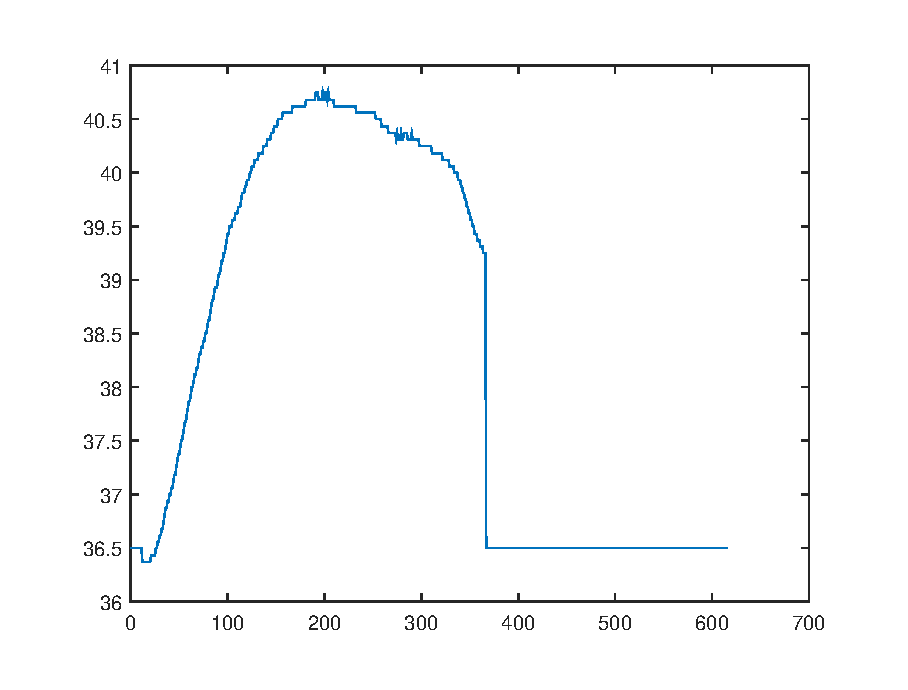
\includegraphics{wykresy/pid2_25_7.eps}
	\caption{Sterowanie obiektu dla $K = 2 , T_i = 25, T_d = 7$}
	\label{lab2eps}
\end{figure}

Dalsz? cz??? projektu zosta?a wykonana na modelu obiektu w ?rodowisku domowym. \
Pierwsz? czynno?ci? jest zasymulowanie stanowiska dla ostatnich nastaw z laboratorium, aby sprawdzi? czy zgrubsza pokrywaj? si? \ref{domporownanie}.
Por�wnuj?c wykres \ref{lab2eps} wraz ze wspomnianym , zauwa?amy podobny z?b przy skoku warto?ci zadanej oraz podobne warto?ci przeregulowania. Sugurej?c si? tymi aspektami mo?na stwierdzi?, ?e model obiektu jest podobny do obiektu rzeczywistego co ?wiadczy o poprawno?ci naszych przekszta?ce?. \

Na wykresie \ref{bleble} przedstawili?my wyniki symulacji dla r�?nych nastaw regulatora wraz z ich 

\begin{figure}[tb]
	\centering
	\begin{tikzpicture}
	\begin{axis}[
	width=0.9\textwidth,
	xmin=0,xmax=615,ymin=36,ymax=41,
	xlabel={$k$},
	ylabel={$Y(k)$},
	xtick={0,50,100,150,200,250,300,350,400,450,500,550,600},
	ytick={36,37,38,39,40,41},
	y tick label style={/pgf/number format/1000 sep=},
	]
	\addplot[blue,semithick] file {wykresy/pidy_2.0000_25.0000_7.0000.txt};
	\addplot[orange,semithick] file {wykresy/pidyzad_38.0000.txt};
	\legend{$Y(k)$,$Y_{zad}$}
	\end{axis}
	\end{tikzpicture}
	\caption{Sterowanie obiektu dla $K = 2, T_i = 25, T_d = 7$}
	\label{domporownanie}
\end{figure}

\begin{figure}[tb]
	\centering
	\begin{tikzpicture}
	\begin{axis}[
	width=0.9\textwidth,
	xmin=0,xmax=615,ymin=36,ymax=41,
	xlabel={$k$},
	ylabel={$Y(k)$},
	xtick={0,50,100,150,200,250,300,350,400,450,500,550,600},
	ytick={36,37,38,39,40,41},
	y tick label style={/pgf/number format/1000 sep=},
	]
	\addplot[blue,semithick] file {wykresy/pidy_3.0000_30.0000_5.0000.txt};
	\addplot[orange,semithick] file {wykresy/pidyzad_38.0000.txt};
	\legend{$Y(k)$,$Y_{zad}$}
	\end{axis}
	\end{tikzpicture}
	\caption{Sterowanie obiektu dla $K = 3, T_i = 30, T_d = 5$}
	\label{dom3}
\end{figure}

Najlepsze przebiegi dla naszego obiektu uzyskali?my stosuj?c nast?puj?ce nastway $K_p = 3 , T_i = 40 , T_d = 5$ , gdzie wskaznik jako?ci $E = 270,0647 $.
